\section{Two pre-registered side experiments}\label{app:e1}
\setcounter{table}{0}\setcounter{figure}{0}\setcounter{equation}{0}
\setcounter{proposition}{0}\renewcommand{\theproposition}{\Alph{section}.\arabic{proposition}}

This appendix reports two experiments that were pre-registered separately and whose outcomes
are not part of the two comparisons of the main text, although the bottleneck networks
appear in the readings of \cref{sec:transfer:amplitude}: a regulariser of the latent
representations, whose unregularised networks are the two-dimensional label-free networks
of \cref{sec:results2d}, and a token bottleneck that reduces the cost of attention.

\subsection{Latent regularisation}\label{app:e1:latent}

Three criteria of \cref{tab:criteria} (K4, E6 and KP6) and the experiment of this
subsection concern the latent vectors of the transformer, the outputs of its encoder, one
per node, which the rest of the paper does not use. Self-supervised representation learning
guards against representational collapse, the mapping of different inputs to nearly
identical latent vectors, with regularisers on the distribution of the latent vectors. The
sketched isotropic Gaussian regulariser SIGReg \cite{Balestriero2025LeJEPA} projects the
latent vectors onto random directions and penalises the mean, over the directions, of the
Epps--Pulley statistic \cite{EppsPulley1983}, which measures how far the distribution of a
projection is from the standard normal one; it was introduced for joint-embedding
predictive architectures (JEPA), self-supervised networks that predict the latent
representation of one part of an input from that of another.

The latent-regularisation run (\cref{tab:runs}) added SIGReg, applied to a learned
projection of the latent vectors (a projection head), to the label-free objective of the
two-dimensional transformer, with the later code, and asked whether it kept the accuracy and
separated the geometries better in latent space (\cref{tab:e1}). The separation was measured
by the silhouette $S\in[-1,1]$ of the instance-mean latent vectors of the 256 validation
instances, grouped into four bins by the quartiles of the first principal component of the
geometry descriptor; $S$ is near zero when the bins overlap and near one when they are well
separated. The accuracy was unchanged within the pre-registered noise guard. The separation
rose in every seed, by \numEOneDeltaMin{} to \numEOneDeltaMax{}, but by less than the
\numEOneFloor{} required in every seed, and the experiment read NO-GO. Untrained networks
that received the geometry descriptor as input separated the bins better than trained
ones, and a linear probe read the descriptor from them perfectly; without that input, or
with its input weights set to zero, untrained networks did not separate the bins at all.
The descriptor is an input feature of every node, so these readings measure the input
rather than anything learned. The unregularised networks of this run are the label-free
networks of the two-dimensional comparison, which reuses them without retraining
(\cref{sec:methods:training}); the regulariser itself plays no part in the results.

Criterion K4 of the July run (\cref{tab:criteria}) concerned the same kind of regulariser
in an earlier setting: three regularisers of the latent distribution, each added to the
energy and the masked-prediction term of the joint-embedding objective (\ref{app:prereg})
and trained for 2,000 steps on 64 instances, with and without the geometry descriptor, were
compared by the standardised effective rank of the latent vectors on 256 instances. The
best raised it by more than the factor of 1.5 at or below which the criterion would have
been triggered.

What accuracy does imply for the latent representation is limited to load cases on a
shared stiffness matrix. Fix one instance, with load vectors $F_1,\dots,F_L$ and solutions
$\Ustar_j=K^{-1}F_j$, and let $\gap(u;F_j)=\Pi_h(u;F_j)-\Pi_h(\Ustar_j;F_j)$ be the energy
gap for the load $F_j$, where $\Pi_h(\cdot\,;F_j)$ is the energy \eqref{eq:energy} with that
load. Let $z_j$ be the network's latent representation of load case $j$, the latent vectors
of all nodes stacked, and let the decoder $D$ be Lipschitz from the latent space, with the
Euclidean norm, to $(\R^{n},\norm{\cdot}_K)$, with constant $\Lambda$.

\begin{proposition}[Separation on a shared operator \cite{CaoSong2026}]\label{prop:sep}
If $\norm{D(z_j)-\Ustar_j}_K\le\beta$ for every $j$, that is, by \cref{lem:exact},
$\gap(D(z_j);F_j)\le\beta^2/2$, then for all $i\neq j$
\begin{equation}
\norm{z_i-z_j} \ge \frac{\norm{\Ustar_i-\Ustar_j}_K-2\beta}{\Lambda}.
\label{eq:sep}
\end{equation}
\end{proposition}

\begin{proof}
By the triangle inequality,
$\norm{\Ustar_i-\Ustar_j}_K\le\norm{\Ustar_i-D(z_i)}_K+\norm{D(z_i)-D(z_j)}_K
+\norm{D(z_j)-\Ustar_j}_K\le2\beta+\Lambda\norm{z_i-z_j}$.
\end{proof}

The bound is informative when the solutions themselves are separated; on sixteen
validation instances of each corpus the smallest separation between the load cases of one
instance, relative to the mean stiffness norm of its solutions, was \numPremiseTwo{} (two
dimensions) and \numPremiseThree{} (three). Across geometries there is no common stiffness
norm, and the natural analogue in a transported metric fails: among the same sixteen
instances, two different geometries had solutions under the same load, normalised to unit
length and interpolated to common coordinates, closer to each other (\numCrossTwo{} and
\numCrossThree{}) than the closest two load cases on a single geometry (\numWithinTwo{} and
\numWithinThree{}). Within a geometry, the rank correlation between the distances of the
latent representations and those of the solutions was \numRhoTwo{} and \numRhoThree{}
(criteria E6 and KP6).

% generated by scripts/make_cmame_material.py from the records; do not edit
\begin{table}[tbp]
\centering
\footnotesize
\setlength{\tabcolsep}{4pt}
\caption{Isotropic Gaussian regularisation of the latent vectors added to the label-free objective (two dimensions, with the later code of \cref{sec:methods:networks}).}
\label{tab:e1}
\resizebox{\ifdim\width>\textwidth\textwidth\else\width\fi}{!}{%
\begin{tabular}{lccccccc}
\toprule
Network & Seeds & \shortstack{Displacement \\ error} & \shortstack{Relative \\ energy gap} & S & Probe R$^2$ & 1-NN & \shortstack{SIGReg statistic \\ (tokens)} \\
\midrule
Label-free & 3 & 0.0634 $\pm$ 0.0031 & 0.0383 $\pm$ 0.0019 & $-$0.039 $\pm$ 0.003 & 0.957 $\pm$ 0.010 & 0.40 $\pm$ 0.05 & 0.18 $\pm$ 0.02 \\
Label-free + SIGReg (head) & 3 & 0.0604 $\pm$ 0.0019 & 0.0365 $\pm$ 0.0008 & $-$0.031 $\pm$ 0.004 & 0.976 $\pm$ 0.002 & 0.44 $\pm$ 0.03 & 0.19 $\pm$ 0.01 \\
Label-free + SIGReg (raw tokens) & 1 & 0.0626 & 0.0384 & $-$0.049 & 0.939 & 0.38 & 0.0021 \\
Untrained, descriptor input & 3 & -- & -- & 0.336 $\pm$ 0.024 & 1.000 $\pm$ 0.000 & 0.97 $\pm$ 0.00 & 0.31 $\pm$ 0.02 \\
Untrained, descriptor weights zeroed & 3 & -- & -- & $-$0.031 $\pm$ 0.002 & 0.198 $\pm$ 0.010 & 0.28 $\pm$ 0.03 & 0.32 $\pm$ 0.01 \\
Untrained, no descriptor input & 3 & -- & -- & $-$0.032 $\pm$ 0.001 & 0.210 $\pm$ 0.004 & 0.26 $\pm$ 0.02 & 0.31 $\pm$ 0.00 \\
\bottomrule
\end{tabular}}

\smallskip
\begin{minipage}{\linewidth}\footnotesize\raggedright
Accuracy criterion (regularised against label-free): displacement $-$4.7\% (noise guard 10\%), relative energy gap $-$4.6\% (noise guard 10\%): not triggered.\par
Effect (S of the regularised network minus S of the label-free network, per seed): +0.009 / +0.014 / +0.002; the pre-registered floor is 0.02 in every seed: not met. Outcome: NO-GO; the regulariser was not adopted.\par
256 validation instances; seed mean $\pm$ sample SD. S: silhouette of the instance-mean latent vectors over four bins, the quartiles of the first principal component of the geometry descriptor; probe R$^2$: linear probe of the geometry descriptor; 1-NN: leave-one-out accuracy of a nearest-neighbour classifier of the bin, chance 0.25 with 4 bins of 64.\par
The geometry descriptor is also a per-node model input, so S, the probe and 1-NN largely read the input back; they are not evidence of learned geometry. Untrained rows (measured after the runs, same instances): models built from the label-free network's configuration at initialisation with the descriptor input; the same models with the descriptor's input weights set to zero; models built without the descriptor input.\par
SIGReg statistic (tokens): the regulariser's statistic evaluated on the latent vectors themselves rather than on the projection head's output (lower is closer to an isotropic Gaussian). The variant that applies the regulariser to the latent vectors directly (raw tokens) ran one seed and is reported only.
\end{minipage}
\end{table}


\subsection{Token bottleneck}\label{app:e1:bottleneck}

To reduce the cost of attention, the bottleneck run (\cref{tab:runs}) tested, under a
separate pre-registration, a token-bottleneck network that pools the nodes into $M=512$ or
$M=1{,}024$ tokens seeded by farthest-point sampling, applies attention to the tokens only,
and decodes each node from a smooth blend of its six nearest tokens. It was trained on the
energy alone, with every other setting as for the transformer (\cref{tab:e2,fig:e2}). It
trained \numTimeBottleneckSpeedup{} times faster per seed (\numTimeBottleneckSeedMin{} h
against \numTimeThreeSeed{} h), but it was less accurate: its in-band relative energy gap
was \numEtwoGapMin{} to \numEtwoGapMax{} times the transformer's and its zero-shot
fine-mesh displacement error \numEtwoFineMin{} to \numEtwoFineMax{} times. Both variants
were dropped under their pre-registered accuracy criterion (\cref{tab:criteria}). Their
amplitudes on the finer mesh, measured after the runs, are in
\cref{tab:amplitude,tab:remesh}.

% generated by scripts/make_cmame_material.py from the records; do not edit
\begin{table}[tbp]
\centering
\footnotesize
\setlength{\tabcolsep}{4pt}
\caption{Token bottleneck against the label-free transformer, which has one token per node, both trained on the energy alone with the same corpus, split, seeds and schedule (three dimensions).}
\label{tab:e2}
\resizebox{\ifdim\width>\textwidth\textwidth\else\width\fi}{!}{%
\begin{tabular}{lccccc}
\toprule
Network & \shortstack{In-band \\ displacement} & \shortstack{In-band relative \\ energy gap} & \shortstack{Fine displacement \\ (zero-shot)} & \shortstack{Step (ms), \\ 12,318 nodes} & \shortstack{Step (ms), \\ 41,367 nodes} \\
\midrule
Label-free transformer & 0.0300 $\pm$ 0.0028 & 0.00912 $\pm$ 0.00228 & 0.258 $\pm$ 0.045 & 1,415 & 14,795 \\
Token bottleneck, M = 512 & 0.106 $\pm$ 0.051 & 0.0348 $\pm$ 0.0226 & 0.463 $\pm$ 0.082 & 27.8 & 49.2 \\
Token bottleneck, M = 1,024 & 0.0892 $\pm$ 0.0096 & 0.0258 $\pm$ 0.0051 & 0.574 $\pm$ 0.059 & 36.9 & 47.5 \\
\bottomrule
\end{tabular}}

\smallskip
\begin{minipage}{\linewidth}\footnotesize\raggedright
M = 512: accuracy criterion, in-band relative energy gap +280.9\% (noise guard 287\%), fine displacement +79.1\% (noise guard 42\%; triggered); speed criterion, fine-mesh step 0.049 s against the 2.0 s limit: not triggered. Outcome: dropped.\par
M = 1,024: accuracy criterion, in-band relative energy gap +183.3\% (noise guard 70\%; triggered), fine displacement +122.0\% (noise guard 33\%; triggered); speed criterion, fine-mesh step 0.047 s against the 2.0 s limit: not triggered. Outcome: dropped.\par
Seeds per network: 3; seed mean $\pm$ sample SD. In-band: the 256 validation instances ($l_c$ = 0.0579--0.0906; the benchmark instances at the two ends of this range have 12,318 and 3,774 nodes); fine: 256 instances at $l_c$ = 0.0374 (41,367 nodes in the benchmark), never trained on. Errors are relative displacement error and relative energy gap.\par
Step time: one label-free training step on one instance of the stated size, NVIDIA GeForce RTX 5090, TF32 on, from a dedicated benchmark (bottleneck: the median over three repetitions of the time of 110 steps minus that of 10 steps, divided by 100, which removes the set-up time; transformer: a single timed step, its set-up included, the mean of its two benchmark measurements, 1,408 / 1,422 ms and 14,793 / 14,798 ms).\par
Noise guard: as in the note to \cref{tab:criteria}, with the label-free transformer as the reference; the pre-registration calls it the resolution.
\end{minipage}
\end{table}


\begin{figure}[tbp]
\centering
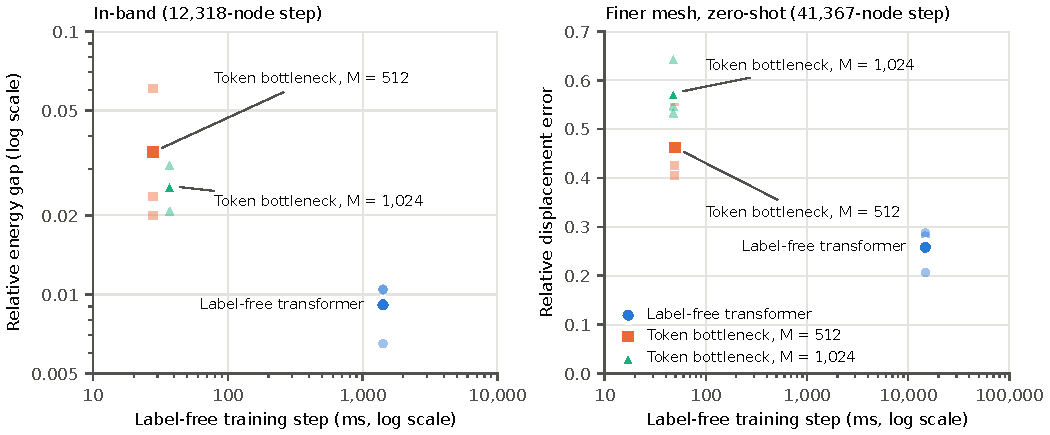
\includegraphics[width=\linewidth]{generated/fig_e2_cost_accuracy.pdf}
\caption{Cost against accuracy of the label-free transformer and the token bottleneck
(three dimensions, three seeds each; faint markers are seeds, ringed markers seed means).
Left: in-band relative energy gap against the time of one training step on an in-band
instance. Right: zero-shot fine-mesh displacement error against the time of one step on a
fine-mesh instance.}
\label{fig:e2}
\end{figure}
